\documentclass[11pt]{article}
\usepackage[a4paper,margin=22mm]{geometry}
\usepackage{amsmath,amssymb,booktabs,array,graphicx,float,hyperref,siunitx,xcolor,microtype}
\hypersetup{colorlinks=true,linkcolor=blue!60!black,citecolor=blue!60!black,urlcolor=blue!60!black}
\sisetup{detect-all=true,per-mode=symbol}
\setlength{\parskip}{0.58em}
\setlength{\parindent}{0pt}
\title{Metglas AMCC-1000 Orthogonal Paraformer Experiment Section for the Updated-Coil Simulator}
\author{Walter Russell optical dynamo updated-coil simulation package}
\date{31 May 2026}

\begin{document}
\maketitle

\begin{abstract}
This experiment section specifies the Metglas AMCC-1000 orthogonal paraformer
measurement and simulation protocol used in the updated-coil dynamic simulator.
It combines the physical AMCC-1000 dimensions, material assumptions, lumped
magnetic equations, resonant state-space model, and simulated waveforms.  The
purpose is to separate measured, falsifiable Metglas behavior from speculative
interpretation: the experiment must determine real coupling \(k\), loaded Q,
core loss, winding capacitance, insulation margin, and B-side extraction
behavior before any high-power operation.
\end{abstract}

\section{Core Dimensions and Material Parameters}
The AMCC-1000 class core constants used by the model are
\[
A_e=\SI{23.0}{cm^2},\quad l_e=\SI{42.7}{cm},\quad
W_a=\SI{42.0}{cm^2},\quad A_p=\SI{966}{cm^4}.
\]
The Rev.07 drawing dimensions used in the technical drawing are
\[
a=\SI{33}{mm},\ b=\SI{40}{mm},\ c=\SI{105}{mm},\
d=\SI{85}{mm},\ e=\SI{106}{mm},\ f=\SI{171}{mm},
\]
with mass \SI{7109}{g} and nominal pack factor \SI{82}{\percent}.
The Metglas 2605SA1 material assumptions are \(B_s=\SI{1.56}{T}\), small
signal \(\mu_r\approx 45000\), ribbon thickness \SI{23}{\micro m}, and
resistivity \(\rho=\SI{1.3e-6}{\ohm m}\).

\resizebox{0.92\textwidth}{!}{%
\begin{tabular}{lrlrrrr}
\toprule
Part & Orientation & Flux axis & Turns & Gap (mm) & Lself (mH) & XL 128 kHz (ohm) \\
\midrule
U\_A & 0.0 & X & 8 & 2.000 & 0.092052 & 74.032 \\
U\_B & 90.0 & Y & 8 & 2.000 & 0.092052 & 74.032 \\
\bottomrule
\end{tabular}
}

\section{Magnetic Circuit and Resonance Equations}
For an explicitly gapped core, the lumped reluctance approximation is
\begin{equation}
\mathcal{R} =
\frac{l_e}{\mu_0\mu_r A_e}+\frac{g}{\mu_0 A_e},
\end{equation}
and therefore
\begin{equation}
L(N,g)=\frac{N^2}{\mathcal{R}}
= \frac{\mu_0N^2A_e}{l_e/\mu_r+g}.
\end{equation}
At resonance,
\begin{equation}
C_0 = \frac{1}{(2\pi f_0)^2L},\qquad X_L=2\pi f_0L.
\end{equation}
For sinusoidal flux density with peak \(B_p\),
\begin{equation}
V_{\rm rms} = \frac{2\pi f N A_e B_p}{\sqrt{2}},
\qquad
B(t)=\frac{L i(t)}{N A_e}.
\end{equation}
The orthogonal transfer model is
\begin{equation}
M=k\sqrt{L_A L_B},
\qquad
v_B(t)=M\frac{di_A}{dt},
\qquad
p_{A\rightarrow B}(t)=v_B(t)i_B(t).
\end{equation}
The matched-load transfer limit follows from the Thevenin result:
\begin{equation}
P_{\max} = \frac{(\omega M I_A)^2}{4R_B}.
\end{equation}

\section{Experimental Method}
\begin{enumerate}
\item Measure U\_A and U\_B separately with an LCR meter over frequency to
obtain \(L\), ESR, self-resonant frequency, and loaded Q.
\item Use a VNA to measure \(S_21\) between U\_A and U\_B at low flux.  Fit
the mutual inductance and coupling coefficient \(k=M/\sqrt{L_AL_B}\).
\item Repeat the measurement at several gaps around \SI{2}{mm} and at
several winding positions to quantify mechanical sensitivity.
\item Drive U\_A at \SI{128}{kHz} through an isolated, current-limited
resonant source.  Measure \(i_A(t)\), \(v_A(t)\), induced \(v_B(t)\), and core
temperature.
\item Add the B4 pickup/load network only after low-power \(k\), Q, and loss are
known.  Verify that the B-side load does not detune the A-side ladder.
\item Increase flux in small steps while logging current, voltage, spectrum,
thermal rise, and any partial-discharge signature.
\end{enumerate}

\section{Simulation Results from the Updated-Coil Run}
The updated run used the solved A/B cable lengths, including equal
\SI{445.293167}{m} end-to-end active C1--C8 cable length.  The center
simulation at \SI{128}{kHz} produced:

\resizebox{\textwidth}{!}{%
\begin{tabular}{lrrl}
\toprule
Metric & RMS/mean & Peak/limit & Unit \\
\midrule
U\_A\_core\_current & 2.478628 & 3.449532 & A \\
U\_B\_core\_current & 3.367880 & 4.758976 & A \\
U\_A\_capacitor\_voltage & 183.020191 & 255.414153 & V \\
U\_B\_capacitor\_voltage & 249.530296 & 352.351148 & V \\
U\_A\_flux\_density & 0.012400 & 0.017257 & T \\
U\_B\_flux\_density & 0.016849 & 0.023808 & T \\
direct\_U\_A\_to\_U\_B\_mutual\_voltage & 14.275697 & 19.908115 & V \\
input\_A4\_to\_U\_A\_mutual\_voltage & 21.629079 & 30.577635 & V \\
output\_U\_B\_to\_B4\_mutual\_voltage & 54.305273 & 76.609354 & V \\
actual\_average\_U\_A\_to\_U\_B\_power & 10.267611 & 58.458069 & W \\
actual\_average\_net\_U\_A\_to\_U\_B\_power & 21.344931 & 22.945421 & W \\
matched\_thevenin\_U\_A\_to\_U\_B\_limit & 8.711158 & 70.991223 & W \\
\bottomrule
\end{tabular}
}

\resizebox{\textwidth}{!}{%
\begin{tabular}{lrrrrr}
\toprule
Case & k & M (uH) & Ipri (Arms) & Voc (Vrms) & Pmax (W) \\
\midrule
dynamic\_U\_A\_to\_U\_B & 0.080 & 7.364140 & 2.475577 & 14.661833 & 8.711158 \\
dynamic\_U\_B\_to\_U\_A & 0.080 & 7.364140 & 3.369146 & 19.954079 & 16.134768 \\
target\_50mT\_U\_A\_to\_U\_B & 0.080 & 7.364140 & 7.067092 & 41.855512 & 70.991223 \\
target\_50mT\_U\_B\_to\_U\_A & 0.080 & 7.364140 & 7.067092 & 41.855512 & 70.991223 \\
\bottomrule
\end{tabular}
}

For the dynamic U\_A to U\_B case, \(k=0.080\),
\(M=\SI{7.364140}{\micro H}\),
\(I_A=\SI{2.475577}{A_{rms}}\), and
\(P_{\max}=\SI{8.711158}{W}\).
At the \SI{50}{mT} target current, the same weak coupling gives only
\SI{70.991223}{W}.  The
near-\SI{10}{kW} orthogonal design point is therefore not achieved by the
low-flux small-signal center; it is an extrapolated high-flux matched-load
condition:

\resizebox{0.88\textwidth}{!}{%
\begin{tabular}{lr}
\toprule
Quantity & Value \\
\midrule
Required B peak & 0.593428 T \\
Selected turns per winding & 12 \\
Primary winding current & 55.917426 Arms \\
Primary winding voltage & 9314.329 Vrms \\
Secondary open-circuit voltage & 745.146 Vrms \\
Matched secondary resistance & 13.881077 ohm \\
Matched secondary current & 26.840365 Arms \\
Matched secondary power & 10000.000 W \\
L self & 0.207116 mH \\
M mutual & 16.569316 uH \\
Resonance C & 7.464586 nF \\
Circulating reactive power & 0.520833 MVAR \\
Parallel AWG10-equivalent bundles & 4 \\
Procurement cable, two windings & 93.840 m \\
\bottomrule
\end{tabular}
}


\begin{figure}[H]
\centering
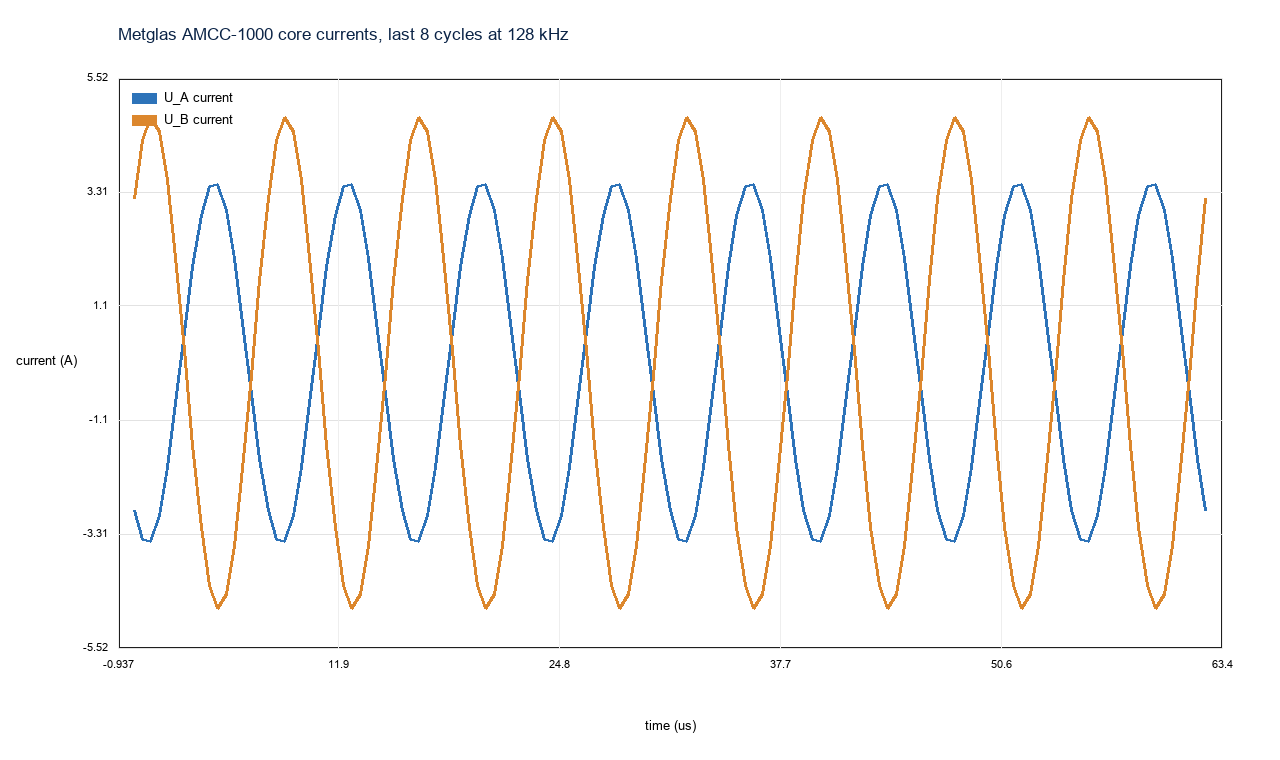
\includegraphics[width=0.94\textwidth]{../figures_updated_coils_20260531/metglas_core_currents.png}
\caption{Updated-coil Metglas $U_A$ and $U_B$ resonant currents over the final eight cycles.}
\label{fig:upd-metglas-currents}
\end{figure}


\begin{figure}[H]
\centering
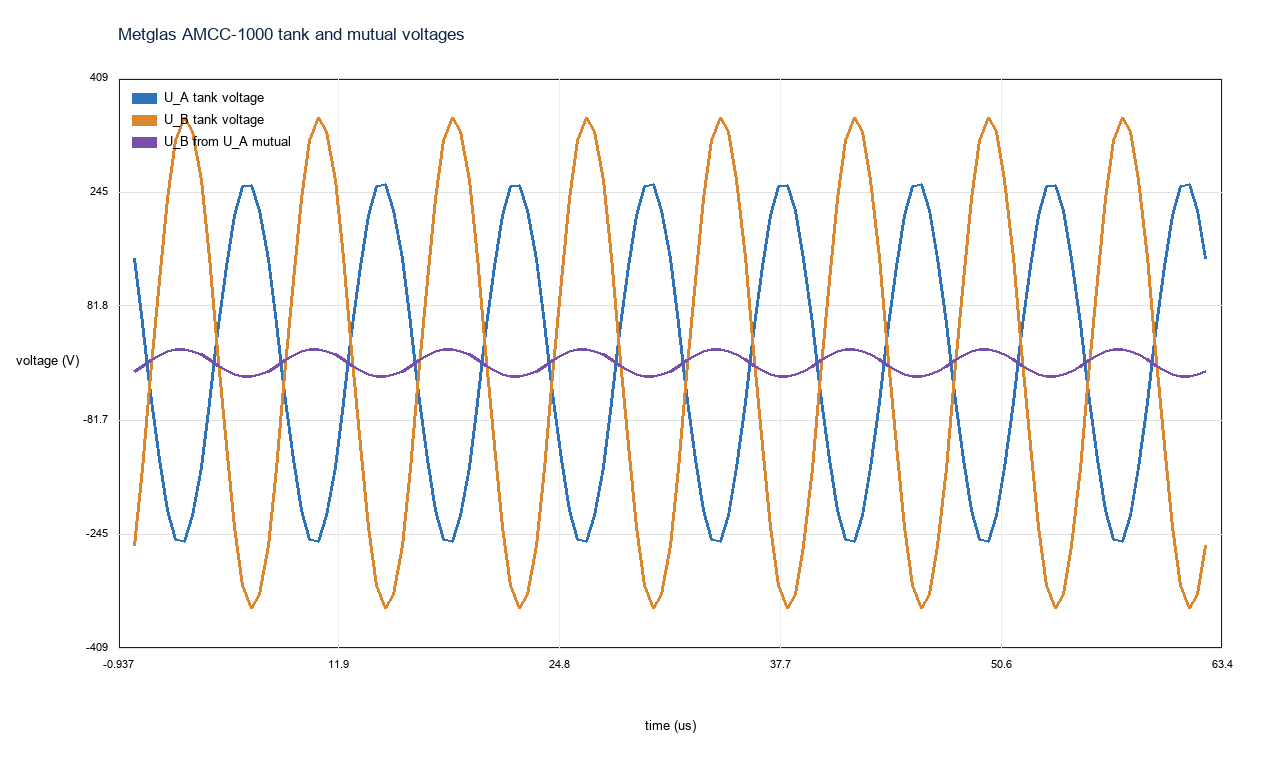
\includegraphics[width=0.94\textwidth]{../figures_updated_coils_20260531/metglas_core_voltages.png}
\caption{Updated-coil Metglas tank voltages and the direct $U_A$ to $U_B$ mutual voltage.}
\label{fig:upd-metglas-voltages}
\end{figure}


\begin{figure}[H]
\centering
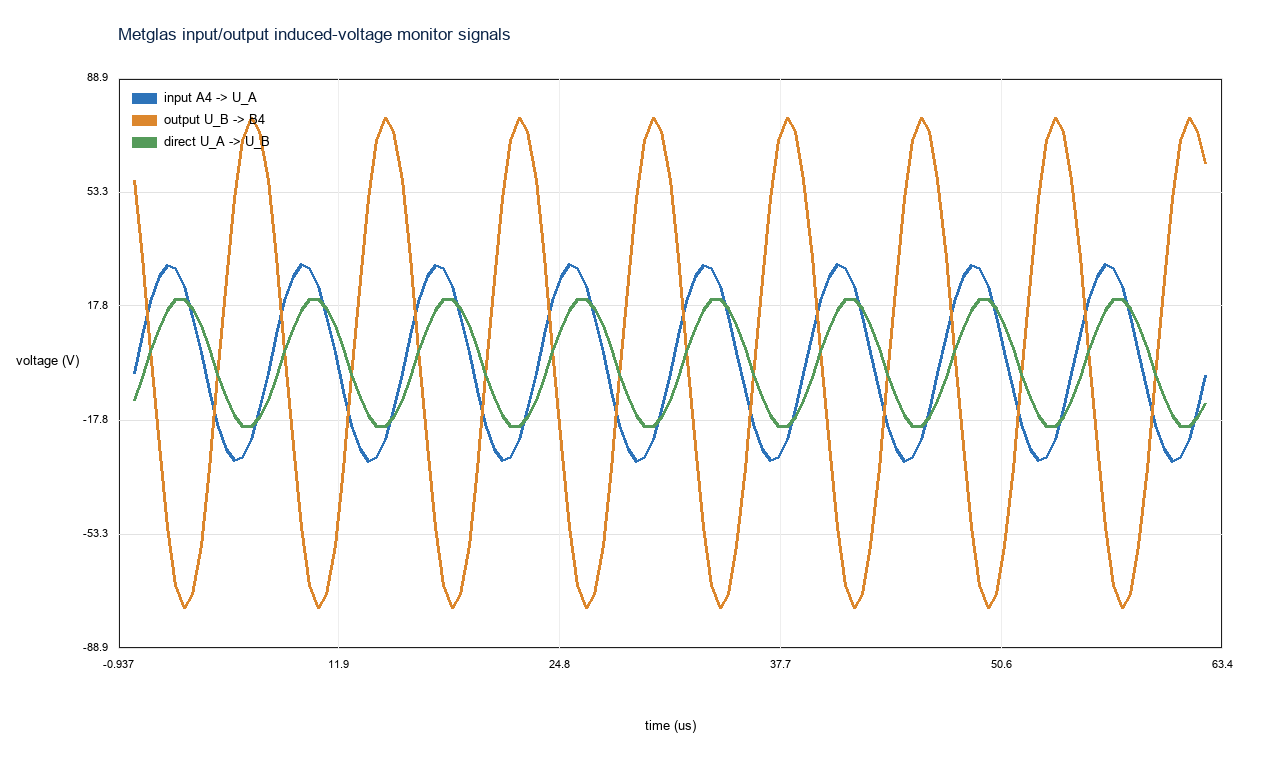
\includegraphics[width=0.94\textwidth]{../figures_updated_coils_20260531/metglas_input_output_signals.png}
\caption{Input and output monitor voltages: A4 into $U_A$, $U_B$ into B4, and direct $U_A$ to $U_B$.}
\label{fig:upd-metglas-io}
\end{figure}


\begin{figure}[H]
\centering
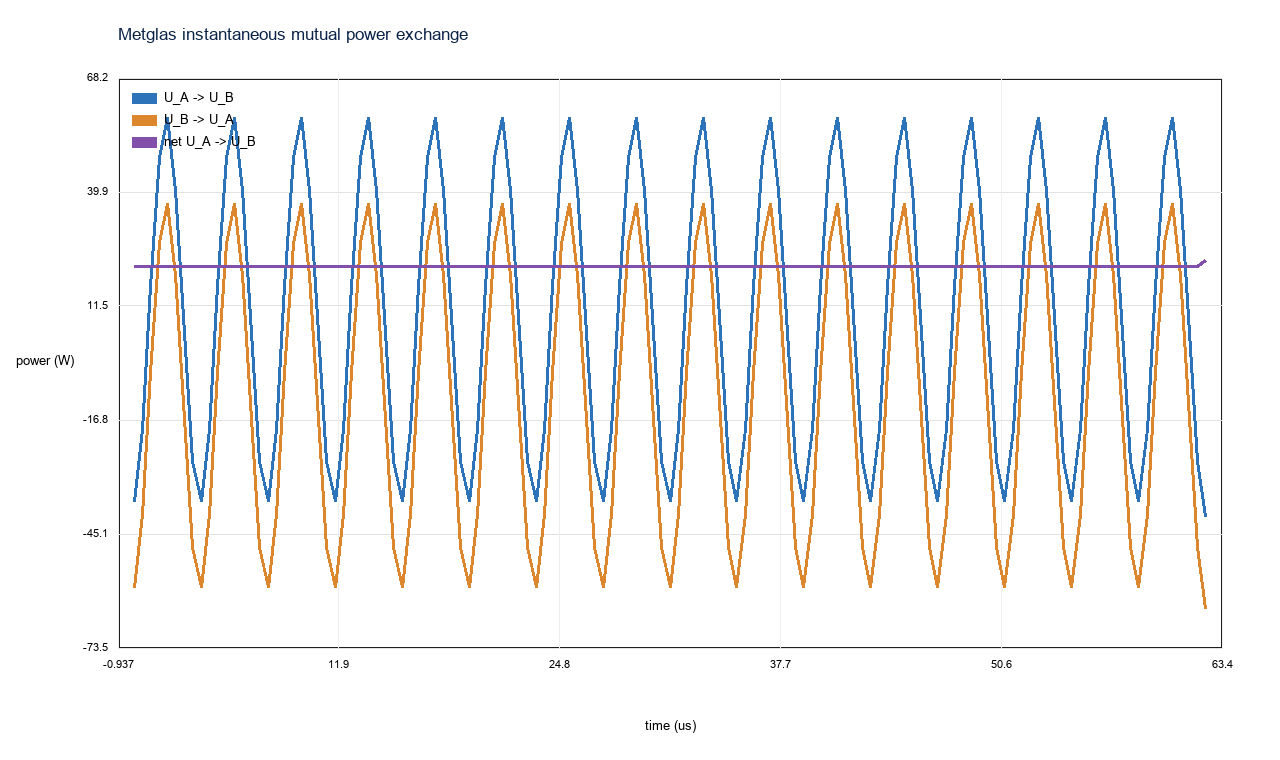
\includegraphics[width=0.94\textwidth]{../figures_updated_coils_20260531/metglas_transferred_power_time.png}
\caption{Instantaneous mutual power exchange and net directional power in the orthogonal Metglas pair.}
\label{fig:upd-metglas-power-time}
\end{figure}


\section{Acceptance Criteria}
The experiment passes the low-power validation stage only if the measured
resonant frequency is within the capacitor trim range, the measured \(k\) agrees
with the fitted model within the experimental uncertainty, the measured core
temperature rise is stable, and the B-side load can be reflected into the pickup
without collapsing Q.  The high-power envelope is rejected if the required flux
density forces saturation, if inter-winding voltage exceeds insulation margin,
or if the measured \(P_{\max}\) does not scale approximately as \(k^2B^2\)
within the safe linear region.

\begin{thebibliography}{9}
\bibitem{grover} F. W. Grover, \emph{Inductance Calculations}, Dover Publications.
\bibitem{dowell1966} P. L. Dowell, ``Effects of eddy currents in transformer windings,'' \emph{Proceedings of the IEE}, 1966.
\bibitem{metglas2605sa1} Metglas Inc., ``2605SA1 Magnetic Alloy,'' product datasheet.
\bibitem{amcc1000} Hitachi Metals / Metglas, ``AMCC1000 product drawing Rev.07.''
\end{thebibliography}

\end{document}
